\documentclass[11pt]{article}
\usepackage[margin=1in]{geometry}
\usepackage{amsmath,amssymb,graphicx,booktabs,hyperref,caption}
\graphicspath{{../plots/}}
\hypersetup{colorlinks=true,linkcolor=black,urlcolor=blue}
\title{\textbf{Do Sentinel Qubits Help Detect Sub-Threshold Eavesdropping in BB84? A Negative Result}}
\author{Sree Charan Desu\\IIIT Andhra Pradesh (RGUKT Ongole)\\\href{mailto:sreecharan309@gmail.com}{sreecharan309@gmail.com}}
\date{October 2026}
\begin{document}
\maketitle
\noindent\fbox{\parbox{\dimexpr\linewidth-2\fboxsep}{\small This paper replaces \texttt{bb84\_fingerprint\_paper.pdf}. That version reported that sentinel-qubit error fingerprints plus a random-forest classifier (AECE) detect sub-threshold eavesdropping and raise the secure key rate. Those results came from a simulator with physics bugs (Section~2). Every number below comes from \texttt{notebook/bb84.ipynb}. Code: \url{https://github.com/sreecharan-desu/bb84-qkd}.}}

\begin{abstract}
BB84 deployments abort when the quantum bit error rate (QBER) goes above about 11\%, so an eavesdropper who stays under that threshold goes unnoticed by the abort rule. We tested a proposed fix: interleave sentinel qubits (20\% of positions, secret from Eve), compare the error statistics of sentinel and key qubits, and classify sessions as noise or attack with a random forest. In a corrected polarization simulation with drift, depolarizing noise, noise bursts and a blind intercept-resend adversary, the sentinel-key QBER difference is at chance as a detector (50.6\% accuracy). With equal average QBER for both classes, the full classifier reaches 65.5\%, and removing every sentinel-based feature leaves 65.1\%. Total QBER alone gives 76.5\% when Eve adds errors on a standard channel. The extra abort rule never increases the secure key rate. We conclude that sentinels add no information against an adversary who can't tell them apart from key qubits.
\end{abstract}

\section{Introduction}
Intercept-resend on a fraction $p$ of qubits adds about $p/4$ to the QBER. With a 4\% noise floor, an Eve at $p=0.1$ sits around 6.3\%, well under the 11\% abort threshold. The hypothesis was that sentinel qubits give a clean noise baseline: if the key qubits show more errors, or a different error pattern, than the sentinels, Eve is present.

The flaw: sentinels only give a baseline if Eve disturbs them differently from key qubits. In BB84, Eve sees the qubits before anyone reveals which are sentinels, so she can't treat them differently.

\section{Errors in the original simulation}
\begin{enumerate}
\item The diagonal basis was encoded at $\pi/2$ and $\pi$ instead of $\pi/4$ and $3\pi/4$, so wrong-basis measurements were deterministic.
\item Eve's resend didn't carry the state she measured.
\item Noise bursts rotated polarization by $\pi$, which leaves a polarization qubit unchanged.
\item Drift was added and then subtracted, so it never acted on the channel.
\item A prototype classifier (\texttt{QT003\_aece.ipynb}) was trained on mocked features, where attack sessions were assigned a higher delta by construction.
\end{enumerate}

\section{Model}
States are prepared at $\theta=\theta_b+(\pi/2)\,x$, with $\theta_+=0$ and $\theta_\times=\pi/4$. Bob, measuring in basis $b$, gets
\[ P(0\mid\varphi,b)=\cos^2(\varphi-\theta_b). \]
Channel, per qubit, in time order: drift $\delta(t)=0.10\sin(2\pi t/400+\varphi_0)+\mathcal N(0,0.02^2)$~rad, not compensated. Depolarizing with probability 0.03 (polarization replaced by a uniformly random one). With probability 0.01, a 10-qubit burst starts, during which the depolarizing probability is 0.5.

Eve: with probability $p$ she measures in a random basis and resends the state she measured. In the clustered variant, her intercept probability is $4p$ for 10 out of every 50 time slots and $p/4$ for the rest. She never knows the sentinel mask.

Features per session (sifted bits only): $\Delta=\mathrm{QBER}_{\text{key}}-\mathrm{QBER}_{\text{sentinel}}$; lag-1 autocorrelation of the sentinel errors, the key errors and all errors; and total QBER. The two-mean Hoeffding band is
\[ \varepsilon=\sqrt{\frac{\ln(2/\alpha)}{2n_k}}+\sqrt{\frac{\ln(2/\alpha)}{2n_s}},\qquad \alpha=0.05. \]
Secure key fraction: $R=1-2h(Q)$, set to 0 when $Q>11\%$.

\section{Validation}
\begin{center}\begin{tabular}{lll}\toprule
check & simulated & expected\\\midrule
wrong-basis $P(1)$ & 0.502 & 0.5\\
noiseless channel, $p$ = 0.2 / 0.5 / 1.0 & 5.2\% / 12.4\% / 25.5\% & 5\% / 12.5\% / 25\%\\
noise-only QBER & 4.06\% & \\
noise + Eve $p$ = 0.1 / 0.2 / 0.3 & 6.3\% / 8.6\% / 11.2\% & \\\bottomrule
\end{tabular}\end{center}

\section{Results}
5 seeds $\times$ 150 noise and 150 attack sessions $\times$ 1,000 qubits, 5-fold cross-validation. Values are means over seeds, with ranges in parentheses.

\begin{table}[h]\centering
\caption{Experiment A: standard channel vs clustered Eve, $p=0.10$.}
\begin{tabular}{ll}\toprule features & accuracy\\\midrule
all & 82.6\% (78.7 to 85.7)\\
total QBER only & 76.5\%\\
$\Delta$ only & 50.6\%\\
all except $\Delta$ & 82.1\%\\
no sentinel-based features & 81.9\%\\\bottomrule\end{tabular}\end{table}

Mean QBER is 4.18\% (noise) vs 6.33\% (Eve), and every Eve session stays under 11\%. Mean $\Delta$ is $-0.0004$ vs $0.0017$, with a standard deviation of 0.022 vs 0.028. No session in either class falls outside the Hoeffding band. Feature importance: total QBER 0.55, every other feature about 0.11.

\begin{table}[h]\centering
\caption{Experiment B: matched QBER (noise depolarizing 3 to 20\% vs Eve $p$ = 0.05 to 0.30; both average about 7.95\%).}
\begin{tabular}{ll}\toprule features & accuracy\\\midrule
all & 65.5\%\\
total QBER only & 50.9\%\\
$\Delta$ only & 51.3\%\\
all except $\Delta$ & 64.1\%\\
no sentinel-based features & 65.1\%\\\bottomrule\end{tabular}\end{table}

The modest above-chance signal comes from the temporal autocorrelation of errors (key-error and all-error autocorrelation each carry about 0.23 importance), and sentinels aren't needed for it.

\begin{table}[h]\centering
\caption{Secure key fraction (mean of 5 seeds).}
\begin{tabular}{lllll}\toprule Eve $p$ & 0 & 0.03 & 0.06 & 0.09 to 0.30\\\midrule
classic (abort $>$ 11\%) & 0.500 & 0.451 & 0.393 & 0.334 falling to 0.007\\
AECE (also abort if flagged) & 0.500 & 0.305 & 0.193 & 0\\\bottomrule\end{tabular}\end{table}

AECE is never above classic. The original idea of ``recovering'' blocks above 11\% is unsound anyway, because $R=1-2h(Q)$ is about zero at 11\% and negative above it.

\begin{figure}[h]\centering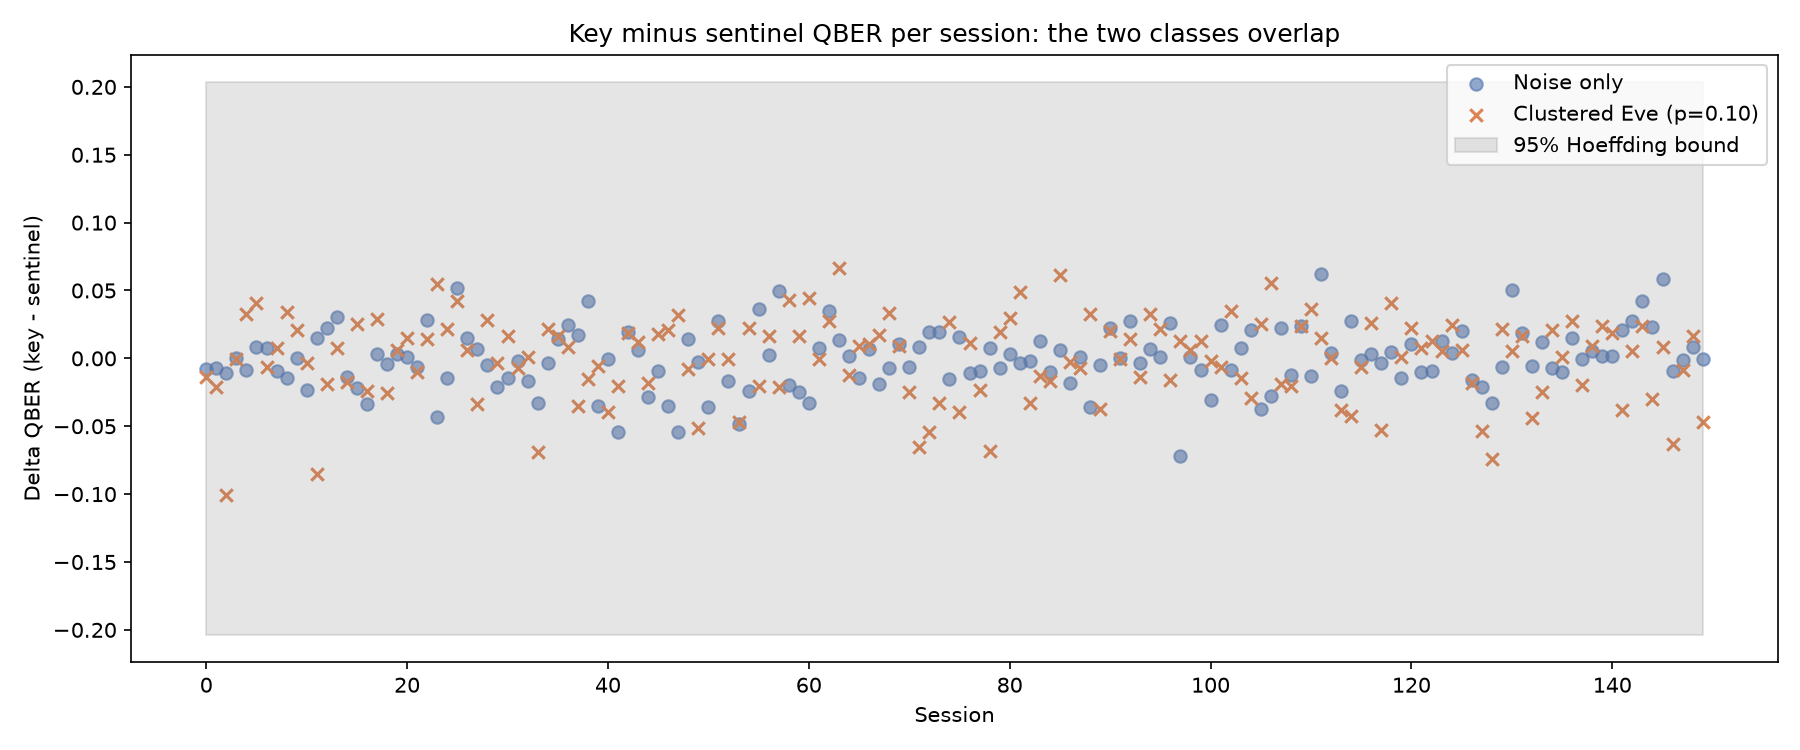
\includegraphics[width=0.8\linewidth]{fingerprint_analysis.png}
\caption{$\Delta$ per session, noise vs clustered Eve ($p=0.10$), with the mean 95\% Hoeffding band. The classes overlap.}\end{figure}
\begin{figure}[h]\centering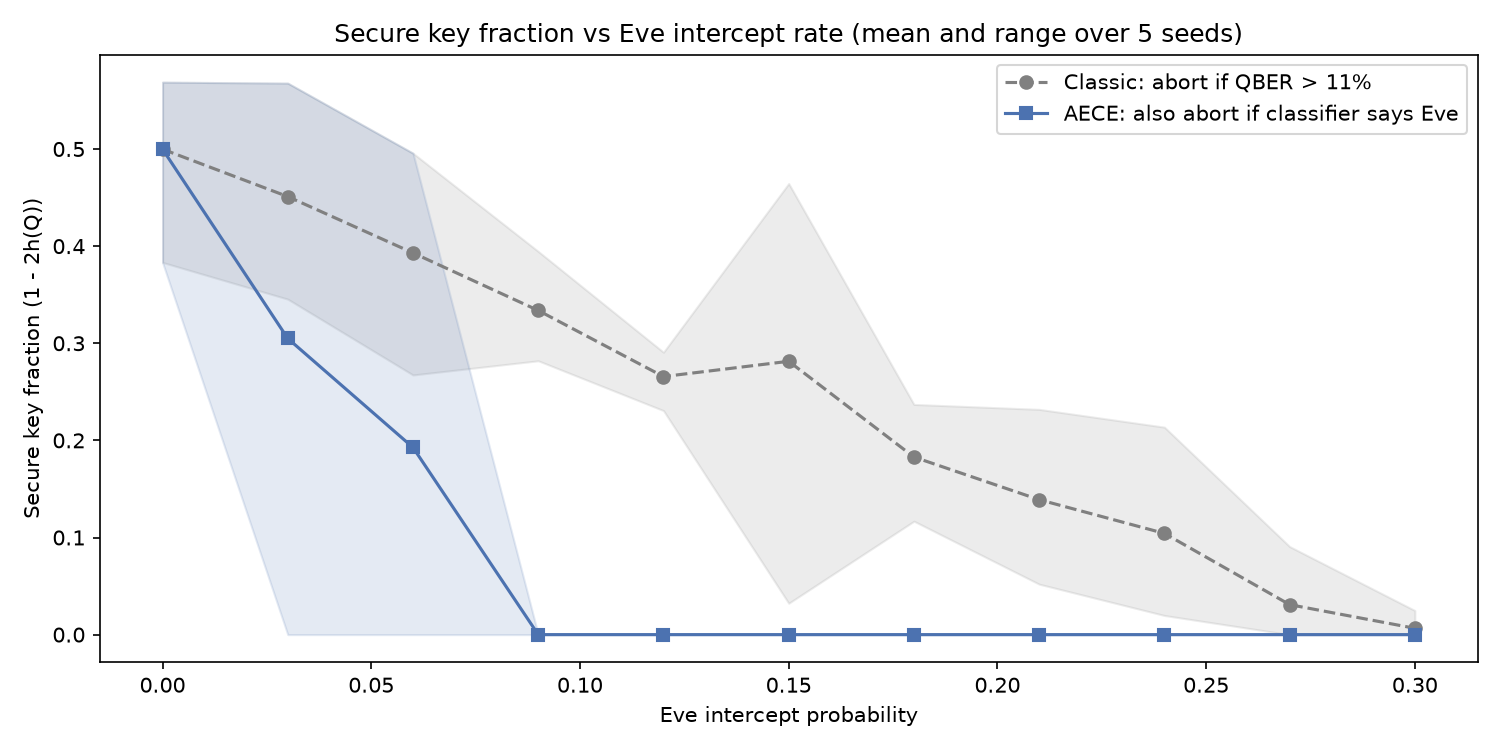
\includegraphics[width=0.8\linewidth]{skr_comparison.png}
\caption{Secure key fraction vs intercept rate, mean and min to max over 5 seeds. AECE is never above classic.}\end{figure}
\begin{figure}[h]\centering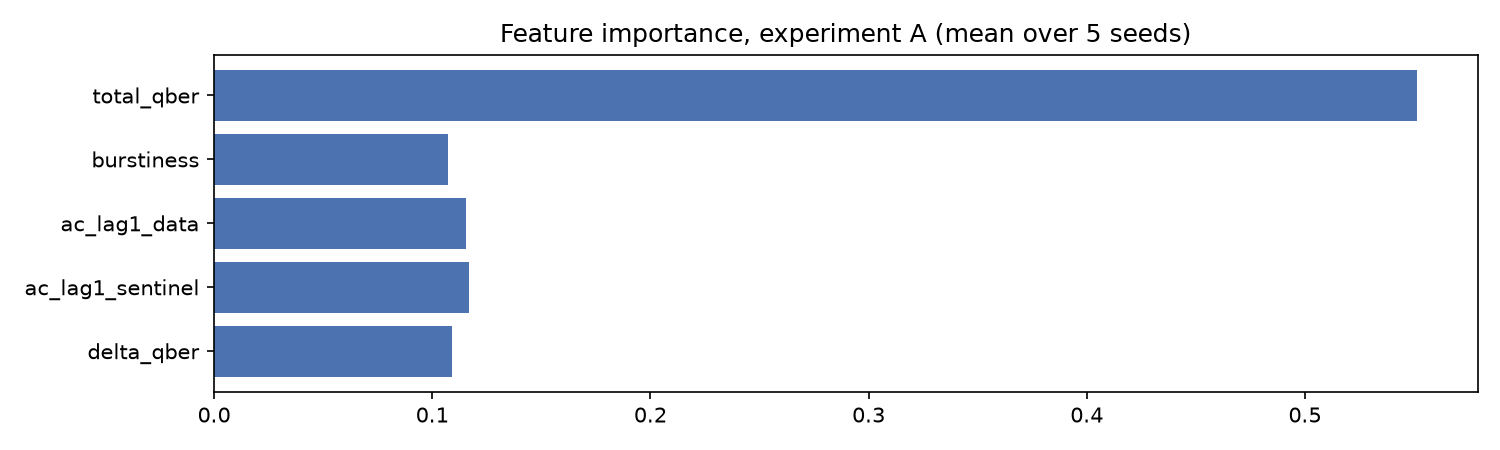
\includegraphics[width=0.7\linewidth]{feature_importance.png}
\caption{Random forest importances in experiment A. Total QBER dominates.}\end{figure}

\section{Discussion and conclusion}
Against an Eve who is blind to sentinels, the sentinel and key qubits are statistically the same sample, so comparing them measures nothing that the overall QBER doesn't. Temporal error structure can carry a weak signal when an attacker clusters interceptions, but that's available without sentinels and depends on the noise model. An extra classifier-based abort can only lower throughput. The proposed AECE doesn't improve on the standard QBER test, and the earlier claims of F1 $>$ 0.94 and 25\% more key are withdrawn.
\end{document}
